% This is a LaTeX thesis template for Monash University.
% to be used with Rmarkdown
% This template was produced by Rob Hyndman
% Version: 6 September 2016

\documentclass{templates/ucdenverthesis}

%%%%%%%%%%%%%%%%%%%%%%%%%%%%%%%%%%%%%%%%%%%%%%%%%%%%%%%%%%%%%%%
% Add any LaTeX packages and other preamble here if required
%%%%%%%%%%%%%%%%%%%%%%%%%%%%%%%%%%%%%%%%%%%%%%%%%%%%%%%%%%%%%%%

\author{Elijah Christensen}
\title{Computational Models of Neural Encoding in Vision and Neurostimulation}
\degrees{BS, University of Washington}
\def\degreetitle{Doctor of Philosophy}
% Add subject and keywords below
\hypersetup{
     %pdfsubject={The Subject},
     %pdfkeywords={Some Keywords},
     pdfauthor={Elijah Christensen},
     pdftitle={Computational Models of Neural Encoding in Vision and Neurostimulation},
     pdfproducer={Bookdown with LaTeX}
}


\bibliography{bib/thesis, bib/jov}

\begin{document}

\pagenumbering{roman}

\titlepage

{\setstretch{1.2}\sf\tighttoc\doublespacing}

\hypertarget{acknowledgements}{%
\chapter*{Acknowledgements}\label{acknowledgements}}
\addcontentsline{toc}{chapter}{Acknowledgements}

Special thanks to Alon Poleg-Polsky for thoughtful discussion and direction and to Gidon Felsen for providing a place to call home.

I would like to thank my support by the Department of Defense (DoD) through the National Defense Science \& Engineering Graduate Fellowship (NDSEG) Program as well as by the Canada First Research Excellence Fund (CFREF) and York University.

\hypertarget{preface}{%
\chapter*{Preface}\label{preface}}
\addcontentsline{toc}{chapter}{Preface}

The material in Chapter \ref{ch:intro} has been submitted to the journal \emph{Journal of Impossible Results} for possible publication.

The contribution in Chapter \ref{ch:litreview} of this thesis was presented in the International Symposium on Nonsense held in Dublin, Ireland, in July 2015.

\clearpage\pagenumbering{arabic}\setcounter{page}{0}

\hypertarget{ch:intro}{%
\chapter{INTRODUCTION}\label{ch:intro}}

Neurological and psychiatric disease represent a significant societal burden in both advanced and developing countries \autocite{Collins:2011ja} and there is a significant need for more effective treatments.
Recent advances in brain stimulation and recording technology have enabled development of long-desired treatment options for many of these diseases in the form of implantable devices that directly stimulate populations of neurons.
Deep brain stimulation (DBS) is one such implantable device wherein patients receive electrical pulses via electrodes that have been implanted in the brain to mitigate their disease symptoms.
DBS has become an established therapy for movement disorders \autocite{Perlmutter:2006kp} as well as epilepsy and psychiatric diseases \autocite{Holtzheimer:2011eq}.
Another group of implantable neurostimulators are neural prosthetics, such as cortical prostheses, which aim to restore sight in patients with congenital or acquired blindness. The body of work presented here makes progress on two unsolved challenges limiting advances in implantable neurostimulators, namely DBS state detection and more accurate cortical encoding of visual stimuli.

\hypertarget{sec:dbs}{%
\section{Deep Brain Stimulation}\label{sec:dbs}}

Deep brain stimulation (DBS) uses a surgically implanted stimulator to apply electrical pulses directly to the brain to mitigate symptoms of neurologic and psychiatric disease. Historically, drugs have been the primary method of treating these diseases, but DBS has emerged as a promising alternative for patients who don't respond to pharmacotherapy. Parkinson's disease (PD) was among the first FDA approved uses of DBS for mitigating the disease's motor symptoms. When employed for treating PD, current best practice for DBS therapy uses constant stimulation even though its therapeutic benefits to motor symptoms are only needed when the patient is awake and trying to move (Fig 1). Current implanted stimulators are used this way because they have no way to detect when stimulation isn't needed, such as when the patient is asleep or when lower levels of stimulation are needed to correct resting tremor. This strategy of constant stimulation, or open-loop stimulation, is less power efficient and comes with side effects such as impaired cognition, speech, gait, and balance (Hariz et al., 2008). However, activating DBS stimulation only when necessary requires a robust method for discerning when the patient's brain needs stimulation or not. For example, a closed-loop DBS system would read out the patient's brain state and only deliver electrical pulses during periods when the patient is awake. Closed-loop DBS is more power efficient and would have less collateral side effects by only stimulating when necessary.

\hypertarget{sec:neuralinterfaces}{%
\section{Neural Interfaces}\label{sec:neuralinterfaces}}

Cortical prosthetics (Fig 2) are a form of neural interface used to restore sight in blind patients(Lorach et al., 2013). These implantable neurostimulators bypass lost or damaged neurons and stimulating their targets as the original neurons otherwise would. Cortical prostheses must reproduce the neural activity patterns that would typically be relayed by naturally by neurons of the LGN and retina when directly stimulating visual cortex. Neural encoding, our understanding of how neurons reformat and represent visual stimuli, is key to this goal of properly restoring sight.

\hypertarget{bottom-up-neural-encoding-models}{%
\subsection{Bottom-up neural encoding models}\label{bottom-up-neural-encoding-models}}

The ultimate test of our knowledge of neural encoding is to predict neural responses to stimuli. For instance, we know the visual cortex receives complex spatiotemporal patterns of light relayed by the retina and reformats these patterns to infer what caused them (i.e.~the identity of the object).

A neuron's receptive field (RF) depicts the properties of an image that modulate that neurons activity. RF's are typically represented in model's by linear filters applied at the first stage of processing.

These filters multiplied by an image and summed predict a given neurons response to that image. The linear RF model was insufficient for predicting several non-linear properties of retinal ganglion cell (RGC) responses to white noise.

Linear-Nonlinear-Poisson (LNP) (Paninski et al., 2004) models are commonly used to predict retinal ganglion cell (RGC) spike rates in responses to image stimuli.
LNP combines a linear spatial filter with a single static non-linearity.
The LNP model captured X variance for white noise stimuli but it doesn't generalize to natural image stimuli.
Generalized Linear Model's (GLM) (Pillow et al., 2008) improve prediction accuracy by accounting for interactions between RGC's and substituting the spatial receptive field with a spatiotemporal receptive field.

\hypertarget{sec:ch1summary}{%
\section{Summary}\label{sec:ch1summary}}

Chapter \protect\hyperlink{ch:mlprimer}{2} provides an introduction to machine learning that serves as a foundation for the technical chapters that follow.
In Chapter 3 we discuss work decoding sleep state using neural network models trained on direct intracranial recordings of human basal ganglia.
Importantly, this model generalizes decoding to patients never seen by the model and may allow new ways to leverage implantable stimulators for therapeutic benefit.

Chapter 4 explores the effects multi-functional objectives (recognize and visualize) on both learned representations and task performance. This work was motivated by the observation that visual processing areas are reactivated during visualization tasks indicating their dual role in visual processing and regenerating stimuli.

Finally, Chapter 5 demonstrates the utility of neural network models as way to explain response properties of individual neurons. We achieved state of the art performance at predicting activity of individual neurons evoked by natural image stimuli in macaque V1 using a convolutional neural network. Furthermore, we used this model generatively to explain response properties of cells outside of Hubel and Wiesel's simple- or complex-cell designations.

\hypertarget{ch:mlprimer}{%
\chapter{MACHINE LEARNING AND COMPUTATIONAL NEUROSCIENCE}\label{ch:mlprimer}}

Despite the importance of computers for conducting machine learning and computational neuroscience research both fields had origins long before contemporary transistor computers. In 1943, inspired by the ``all-or-none'' nature of neural activity, Warren McCulloch (neuroscientist) and Walter Pitts (logician) formalized a simple mathematical definition of a neuron \autocite{McCulloch:1943vq}.
McCulloch and Pitts neurons became the fundamental unit of artificial neural networks (ANN). These artificial neurons, often referred to as (artificial) units, reproduce several key properties of real neurons (Figure \ref{fig:fig2-1}A ). Biological neurons receive input from many other neurons via connections (e.g.~synapses) to its dendrites. These synaptic inputs are summated at the soma where the net dendritic input increases or decreases the neurons membrane potential (Fig \ref{fig:fig2-1}A). If the net dendritic input shifts the membrane potential beyond a certain threshold (e.g.~the threshold potential) the neuron will fire action potentials.

\hypertarget{sec:artificialunits}{%
\section{Artificial Units}\label{sec:artificialunits}}

Artificial units (Fig \ref{fig:fig2-1}B) are the basic building block of artificial neural networks. Each artificial unit receives input represented as a sequence of inputs \(x_i\) and each input has a corresponding synaptic weight \(w_i\). The membrane potential \(z\) of the artificial unit is represented by adding net dendritic input to a scalar bias term \(b\) which represents intrinsic excitability. Finally, the threshold non-linear response of biological neurons is captured by passing the units membrane potential \(z\) through an activation function \(g\) which gives the unit output firing rate, or ``activation'', \(a\).

\[
a_j = g(z_j) = g(x_i \cdot w_{i,j} + b_j)
\]

\hypertarget{sec:layers}{%
\section{Layers}\label{sec:layers}}

Just as the brain is comprised of more than one neuron, most models make use of many artificial units. Similar to the laminar organization of the neocortex, artificial neural networks (ANN) group individual units together in layers (Fig \ref{fig:fig2-1}C). The artificial units within a layer collectively operate on a shared input and the layers output consists the collective activations of its constituent artificial units. ANN layers in a model between the inputs (x) and final outputs (y) are often referred to as ``hidden'' layers. The layers of an ANN are often considered analogous to a population of neurons in regions of the brain which perform similar functions. For instance, primary visual cortex (V1) contain a population of neurons which receive visual inputs from the retina (relayed by LGN). As a population of neurons, V1 processes this visual input and this processed visual information is then relayed to area V2 for subsequent processing.

\begin{figure}

{\centering 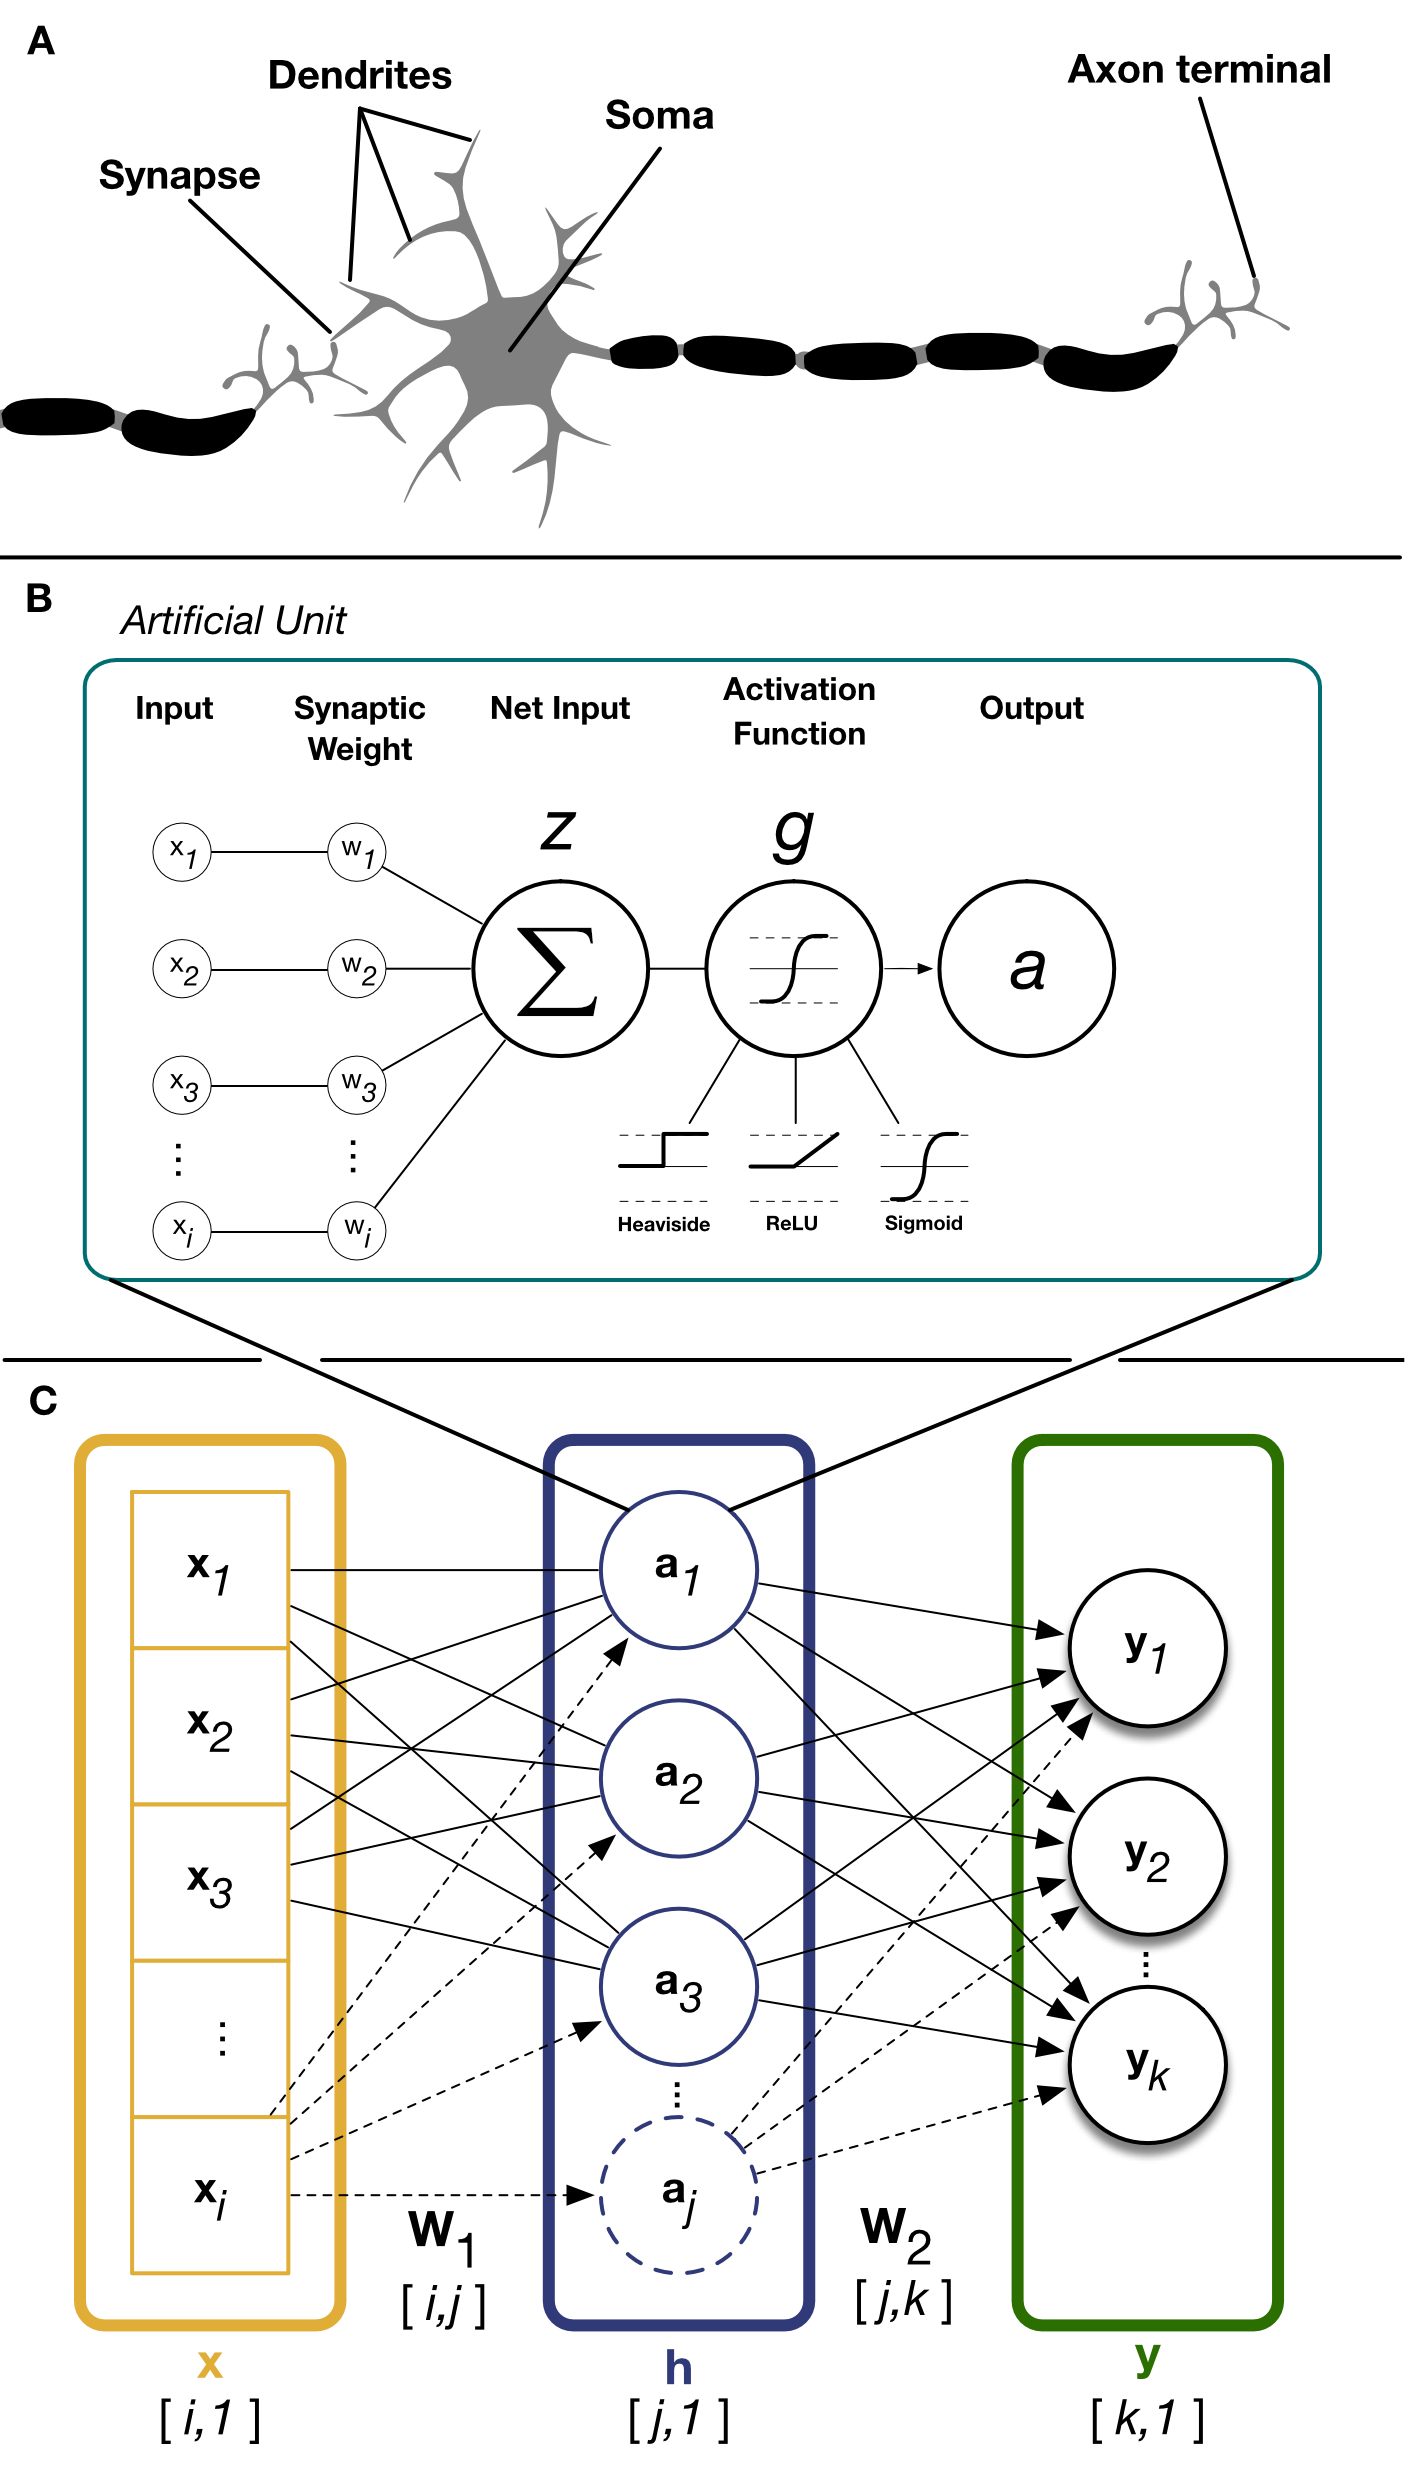
\includegraphics[width=0.75\linewidth]{img/figure_2.1v2} 

}

\caption{Real neurons and artificial units}\label{fig:fig2-1}
\end{figure}

\hypertarget{sec:modarchetypes}{%
\section{Model Archetypes}\label{sec:modarchetypes}}

Deep artificial neural network models typically have multiples of these layers stacked one after the other, such that the outputs of one layer become the inputs for the subsequent layer. Deep ANN models are often constructed for a specific purpose, or to perform a specific task. Models are often categorized based on purported task and the structure of the inputs it uses to accomplish this task. For instance, many computer vision researchers train models which, given an image, categorize the object in the image.

\hypertarget{sec:classifiers}{%
\subsection{Classifiers}\label{sec:classifiers}}

Classifiers are a class of models that attempt to predict the best category that describes the input from a discrete number of categories. For example, a classic machine learning exercise has been to train a model to predict the category of an object depicted in an image. MNIST, Fashion-MNIST \autocite{Xiao:2017wj}, CIFAR10/100 \autocite{Krizhevsky:2009tr} and ImageNet are examples of large labeled image datasets that have been historically popular for evaluating a model's classification performance. Classifiers are not specific image tasks and can be used on any discrete labeling task. For instance, in Chapter 3 we trained an ANN classifier to predict behavioral sleep state in human PD patients based on features from local field potential spectral decompositions.

\hypertarget{sec:regressors}{%
\subsection{Regressors}\label{sec:regressors}}

Regressors use their inputs and attempt to predict a continuous value purportedly derived from the input. Recently, neural network models have been used as functional models of the visual system. These models use images to predict neuronal firing rates observed in animals after viewing the same image and has been used to successfully for predicting stimulus evoked activity in retina \autocite{NIPS2016_6388} and Inferior Temporal cortex (IT) \autocite{Yamins:2014gi}. We successfully utilized a convolutional neural network regressor model to predict firing responses for populations of neurons in macaque primary visual cortex (V1) which is the subject of Chapter 5.

\hypertarget{sec:autoencoders}{%
\subsection{Autoencoders}\label{sec:autoencoders}}

Autoencoders are a special class of models which attempt to predict their inputs. This is a trivial task if each the intermediate hidden layers have similar dimensionality as the input and output; the model can simply learn to copy the input into the output. Instead, these models are more often configured to have far few dimensions in their hidden layers. In this configuration the only way to successfully perform the task is to exploit information redundancy in the input to compress the input while retaining as much information as possible.

\hypertarget{sec:architectures}{%
\section{Layer Architectures}\label{sec:architectures}}

Training an ANN model using machine learning typically requires three components. These components are 1) the model's layer architecture, 2) objective or loss function, and 3) the models learning rules. The layer architecture of a model explicitly specifies how the artificial units, organized in layers, are connected from input to output. There are a wide variety of layers to choose from when constructing a deep ANN but for the sake of brevity only descriptions of layer architectures used in this work will be provided.

\hypertarget{sec:all2all}{%
\subsection{All-to-all}\label{sec:all2all}}

All-to-all layers are the simplest and oldest of layer architectures. In all-to-all layers, every input is connected to every unit in the layer. We can describe this ANN layer mathematically by vectorizing the previous equation wherein inputs and output firing rates are represented as vectors \((x_i,a_j)\) instead of scalars \((x,a)\):

\hypertarget{sec:lossfunc}{%
\section{Loss Function}\label{sec:lossfunc}}

Loss or cost functions ( \(J\) ) are mathematical definitions of the goal of the learning system. The loss function is used to calculate a scalar metric quantifying the models' task performance as a function of its output. Loss functions can take any form mathematically as long as they are 1) differentiable and 2) convex. Reconstruction error (sum of squared pixel errors) were traditionally used for training models which attempt to generate a particular image. We can express the sum squared pixel loss between an image \(\hat{y}\) and the target reference \(y\) as:

\[
J(y,\hat{y}) = \sum (y-\hat{y})^2
\]

Objective functions don't have to depend on a particular dataset or task. For instance, sparse coding models use activation sparseness and reconstruction error as their objective function to learn sparse representations. When minimized over images of natural scenes they learn a set of basis functions that resemble localized receptive fields of simple cells in primary visual cortex \autocite{Olshausen:1996kc}

\hypertarget{sec:learningrules}{%
\section{Learning Rules}\label{sec:learningrules}}

Once a model's architecture and objective function are specified ``training'' it is simply optimizing the parameters of each layer to improve its loss. The algorithm for how to iteratively update the ANN model parameters to minimize loss was first demonstrated by Rumelhart \autocite{Rumelhart:1986er} and it is a simple 2 step process:

\begin{enumerate}
\def\labelenumi{\arabic{enumi})}
\tightlist
\item
  Forward pass: Use a batch of \(x\) input values to calculate the predicted outputs \(\hat{y}\)
\item
  Backpropogation: Use prediction error to update weights and biases
\end{enumerate}

To illustrate this process, we will derive it for a simple 2-layer ANN. For simplicity, we change notation when describing deep ANN with multiple layers such that variable and function subscripts denote the variable or function's corresponding layer NOT matrix or vector dimensions. For instance, we define the output activations of the lth layer in a model comprised of sequentially stacked all-to-all layers as:

\[
a_l = g(a_{l-1} \cdot W_l + b_l)
\]

\hypertarget{sec:fwdpass}{%
\subsection{Forward Pass}\label{sec:fwdpass}}

First, we pass a batch of training example inputs (\(x\)) through the model to get a batch of output classifications (\(\hat{y}\)). Given our simple feedforward layer defined above, the full equation for the models output is given by:

\[
\hat{y} = g(W_2 \cdot g(W_1 \cdot x +b_1) + b_2)
\]

Our loss function \(J\) defines how to evaluate the model's performance as a function of the model's predicted and target values. The target value is also sometimes referred to as the teaching signal, as it's used to teach the model the correct output for a given input. For this example, we'll use sum-squared-error:

\[
J(y,\hat{y}) = \sum (y-\hat{y})^2
\]

\hypertarget{sec:backprop}{%
\subsection{Backpropagation}\label{sec:backprop}}

To derive the gradient of the loss function with respect to the model parameters (\(\nabla_{\theta} J\)) we take a partial derivative of the objective function with respect to the models parameters:

\[
\nabla_{\theta} J = \frac{\partial J(\theta ; y, \hat{y})}{\partial \theta}
\]

\hypertarget{sec:optimizers}{%
\section{Optimizers}\label{sec:optimizers}}

Once we know the gradient of each weight with respect to the loss, we simply need to adjust the weights of the model in the direction specified by the weight gradient. Continually descending the gradient of the loss function should theoretically result in the optimal weights for performing the model's task.

\hypertarget{sec:ch2summary}{%
\section{Summary}\label{sec:ch2summary}}

The purpose of this chapter is not to exhaustively cover the field of machine learning but instead to serve as a brief primer of concepts and terms you will encounter in subsequent chapters. Chapter 2 uses an ANN classifier comprised of fully-connected layers to predict sleep states from LFP spectral decompositions. Chapter 3 utilizes a convolutional autoencoder/classifier hybrid model to test hypotheses about computational objectives employed in primate ventral stream visual representations.
Finally, Chapter 4 uses a convolutional neural network (CNN) to directly regress neuronal activity in macaque primary visual cortex.
Hopefully, you can appreciate the similarities between artificial neural networks and the biological neural networks that inspired them. If nothing else, remember that using machine learning to train ANN models hinges on three components:

\begin{enumerate}
\def\labelenumi{\arabic{enumi})}
\tightlist
\item
  Model architecture
\item
  Loss function
\item
  Learning rules
\end{enumerate}

All three components influence both transient and final model performance.

\hypertarget{ch3:jsr}{%
\chapter{PREDICTING SLEEP STATE IN HUMAN PD PATIENTS}\label{ch3:jsr}}

\begin{itemize}
\item
  The contents of this chapter are available in \href{https://doi.org/10.1111/jsr.12806}{Inferring sleep stage from local field potentials recorded in the subthalamic nucleus of Parkinson's patients.}\footnote{This chapter was previously published in \autocite{Christensen:2019ik} Journal of Sleep Research and is included with permission from the copyright holder}
\item
  {[}\href{http://www.jzlab.org/Christensen_JSleepResearch2018_LFP_ANN_DBS.pdf}{pdf}{]} {[}\href{https://github.com/jzlab/sleep_net}{Source Code}{]}
\end{itemize}

\hypertarget{abstract}{%
\section*{Abstract}\label{abstract}}
\addcontentsline{toc}{section}{Abstract}

Parkinson's disease (PD) is highly comorbid with sleep dysfunction. In contrast to motor symptoms, few therapeutic interventions exist to address sleep symptoms in PD. Subthalamic nucleus (STN) deep brain stimulation (DBS) treats advanced PD motor symptoms and may improve sleep architecture. As a proof of concept toward demonstrating that STN‐DBS could be used to identify sleep stages commensurate with clinician‐scored polysomnography (PSG), we developed a novel artificial neural network (ANN) that could trigger targeted stimulation in response to inferred sleep state from STN local field potentials (LFPs) recorded from implanted DBS electrodes. STN LFP recordings were collected from nine PD patients via a percutaneous cable attached to the DBS lead, during a full night's sleep (6--8 hr) with concurrent polysomnography (PSG). We trained a feedforward neural network to prospectively identify sleep stage with PSG‐level accuracy from 30‐s epochs of LFP recordings. Our model's sleep‐stage predictions match clinician‐identified sleep stage with a mean accuracy of 91\% on held‐out epochs. Furthermore, leave‐one‐group‐out analysis also demonstrates 91\% mean classification accuracy for novel subjects. These results, which classify sleep stage across a typical heterogenous sample of PD patients, may indicate spectral biomarkers for automatically scoring sleep stage in PD patients with implanted DBS devices. Further development of this model may also focus on adapting stimulation during specific sleep stages to treat targeted sleep deficits.

\hypertarget{ch4:intro}{%
\chapter{MODELS OF THE VENTRAL STREAM THAT CATEGORIZE AND VISUALIZE IMAGES}\label{ch4:intro}}

\hypertarget{abstract-1}{%
\section*{Abstract}\label{abstract-1}}
\addcontentsline{toc}{section}{Abstract}

The ventral stream (VS) of visual cortex begins in primary visual cortex (V1), ends in inferior temporal cortex (IT), and is essential for object recognition.
Accordingly, the long-standing belief in the field is that the ventral stream could be understood as mapping visual scenes onto neuronal firing patterns that represent object identity(Felleman and Van Essen, 1991).
Supporting that assertion, deep convolutional neural networks (DCNN's) trained to categorize objects in natural images develop intermediate representations that resemble those in primate VS(Cadieu et al., 2014; Güçlü and van Gerven, 2015; Yamins et al., 2014; Yamins and DiCarlo, 2016).
However, several recent findings appear at odds with the object recognition hypothesis.
VS and other visual areas are also engaged during visualization of both prior experience and novel scenes (O'Craven and Kanwisher, 2006; Stokes et al., 2009), suggesting that the VS can generate visual scenes, in addition to processing them as inputs. Furthermore, non-categorical information, about object positions, sizes, etc. is also represented with increasing explicitness in late VS areas V4 and IT(Hong et al., 2016).
This is not necessarily expected in a ``pure'' object recognition system, as the non-categorical information is not necessary for the categorization task. Thus, these recent findings challenge the long-held object recognition hypothesis of ventral stream and raise the question: What computational objective best explains VS physiology? \autocite{Richards}

To address that question, we pursued a recently-popularized approach and trained deep neural networks to perform different tasks: we then compared the trained neural networks' responses to image stimuli to those observed in neurophysiology experiments3-5,8, to see which tasks yielded models that best matched the neural data. We trained our networks to perform one of two visual tasks: a) recognize objects; or b) recognize objects while also retaining enough information about the input image to allow its reconstruction. We studied the evolution of categorical and non-categorical information representations along the visual pathway within these models, and compared that evolution with data from monkey VS. Our main finding is that neural networks optimized for task (b) provide a better match to the representation of non-categorical information in the monkey physiology data than do those optimized for task (a). This suggests that a full understanding of visual ventral stream computations might require considerations other than object recognition.

\hypertarget{materials-and-methods}{%
\section{Materials and Methods}\label{materials-and-methods}}

\hypertarget{dataset-and-augmentation}{%
\subsection{Dataset and augmentation}\label{dataset-and-augmentation}}

We constructed images of clothing items superimposed at random locations over natural image backgrounds. To achieve this goal, we used all 70,000 images from the Fashion MNIST dataset, a computer vision object recognition dataset comprised of images of clothing articles from 10 different categories. We augmented this dataset by expanding the background of the image two-fold (from 28x28 pixels to 56x56 pixels) and drawing dx and dy linear pixel displacements from a uniform distribution spanning 75\% of the image field \{-11,11\}. Images were then shifted according the randomly drawn dx and dy values. After applying positional shifts, the objects were superimposed over random patches extracted from natural images from the BSDS500 natural image dataset to produce simplified natural scenes which contain categorical (1 of 10 clothing categories) and non-categorical (position shifts) variation. Random 56x56 pixel patches from the BSDS500 dataset were gray scaled before the shifted object images were added to the background patch (Fig 1A). All augmentation was performed on-line during training. That is, every position shift and natural image patch was drawn randomly every training batch instead of pre-computing shifts and backgrounds. This allows every training batch to be composed of unique examples from the dataset and prevents overfitting.

\hypertarget{ch5:jov}{%
\chapter{PREDICTING SINGLE NEURUON RESPONSES IN MACAQUE V1}\label{ch5:jov}}

\begin{quote}
The contents of this chapter are available in \href{https://doi.org/10.1167/19.4.29}{Using deep learning to probe the neural code for images in primary visual cortex}\footnote{This chapter was previously published in \autocite{Kindel:2019et} \emph{Journal of Vision} and is included with permission from the copyright holder}
\end{quote}

\begin{itemize}
\tightlist
\item
  {[}\href{https://github.com/jzlab/v1_predictor}{Source Code}{]}
\end{itemize}

\hypertarget{abstract-2}{%
\section*{Abstract}\label{abstract-2}}
\addcontentsline{toc}{section}{Abstract}

Primary visual cortex (V1) is the first stage of cortical image processing, and major effort in systems neuroscience is devoted to understanding how it encodes information about visual stimuli. Within V1, many neurons respond selectively to edges of a given preferred orientation: These are known as either simple or complex cells. Other neurons respond to localized center--surround image features. Still others respond selectively to certain image stimuli, but the specific features that excite them are unknown. Moreover, even for the simple and complex cells---the best-understood V1 neurons---it is challenging to predict how they will respond to natural image stimuli. Thus, there are important gaps in our understanding of how V1 encodes images. To fill this gap, we trained deep convolutional neural networks to predict the firing rates of V1 neurons in response to natural image stimuli, and we find that the predicted firing rates are highly correlated (\(CC_{norm}\) = 0.556 ± 0.01) with the neurons' actual firing rates over a population of 355 neurons. This performance value is quoted for all neurons, with no selection filter. Performance is better for more active neurons: When evaluated only on neurons with mean firing rates above 5 Hz, our predictors achieve correlations of \(CC_{norm}\) = 0.69 ± 0.01 with the neurons' true firing rates. We find that the firing rates of both orientation-selective and non-orientation-selective neurons can be predicted with high accuracy. Additionally, we use a variety of models to benchmark performance and find that our convolutional neural-network model makes more accurate predictions.

\hypertarget{introduction}{%
\section{Introduction}\label{introduction}}

Our ability to see arises because of the activity evoked in our brains as we view the world around us. Ever since Hubel and Wiesel (1959) mapped the flow of visual information from the retina to thalamus and then cortex, understanding how these different regions encode and process visual information has been a major focus of visual systems neuroscience. In the first cortical layer of visual processing---primary visual cortex (V1)---Hubel and Wiesel identified neurons that respond to oriented edges within image stimuli. These are called simple or complex cells, depending on how sensitive their responses are to shifts in the position of the edge. The simple and complex cells are well studied (Lehky, Sejnowski, \& Desimone, 1992; David, Vinje, \& Gallant, 2004; Montijn, Meijer, Lansink, \& Pennartz, 2016). However, many V1 neurons are neither simple nor complex cells, and the classical models of simple and complex cells often fail to predict how those neurons will respond to naturalistic stimuli (Olshausen \& Field, 2005). Thus, much of how V1 encodes visual information remains unknown. We use deep learning to address this longstanding problem.

\hypertarget{methods}{%
\section{Methods}\label{methods}}

\hypertarget{experimental-data}{%
\subsection{Experimental Data}\label{experimental-data}}

Neural activity was recorded in monkeys' V1 as they were shown a series of images (Fig \ref{fig:5-1}A). The image set contains 270 circularly cropped natural images (Fig \ref{fig:5-1}B). (C) The response of a single neuron over repeated presentations of an image. Ticks indicate the neuron's spiking; each row corresponds to a different image-presentation trial. During the response window, the firing rate is computed and then averaged over trials to yield the average response \(A_{n,i}\) used in our analysis. (D) The neuron responds to image stimuli with a latency of ∼50 ms from the image onset at t = 0, as seen in the peristimulus time histogram (firing rate plotted against time, averaged over all 270 images).

\begin{figure}

{\centering 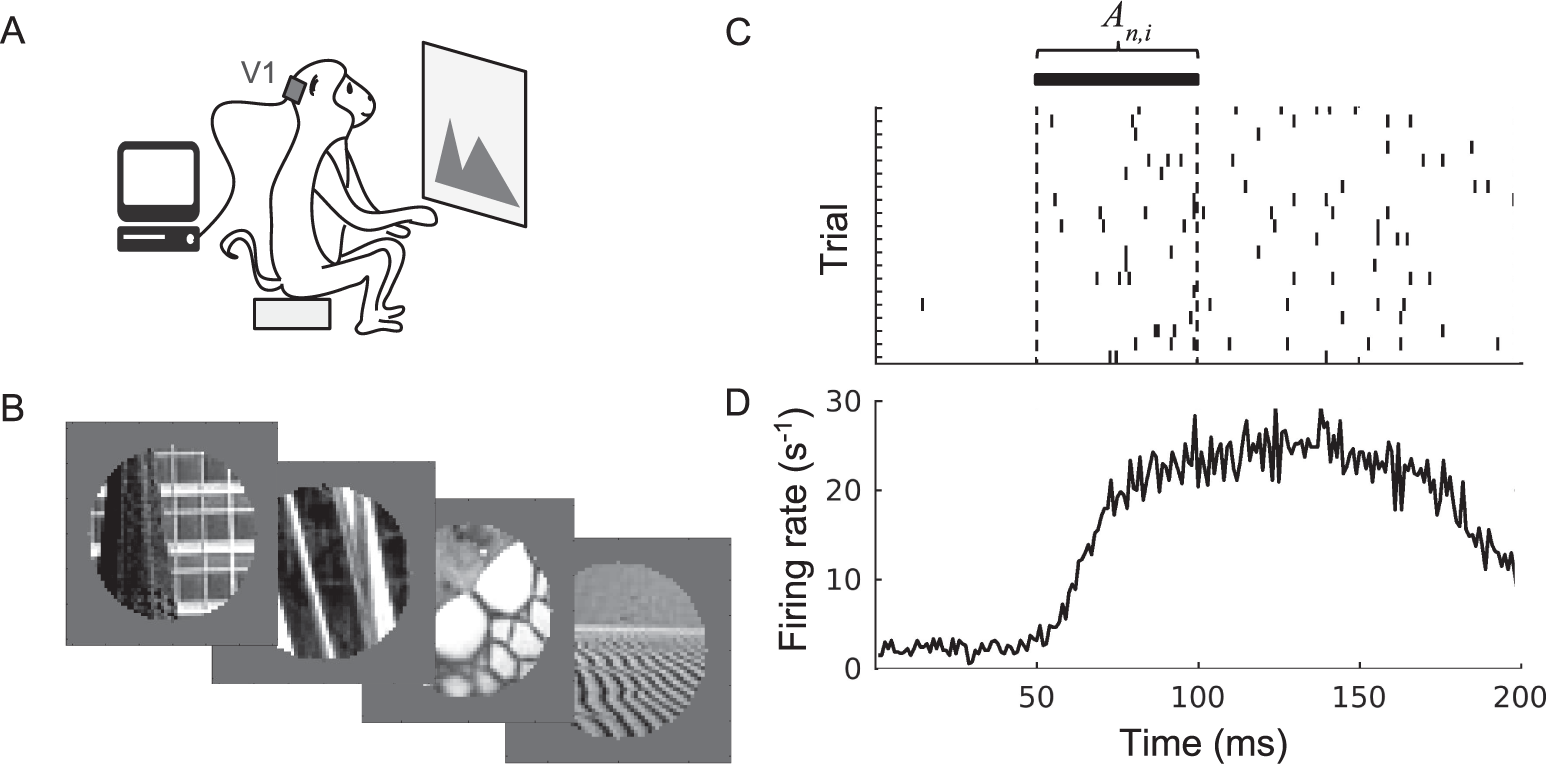
\includegraphics[width=0.75\linewidth]{img/figure_5.1} 

}

\caption{Experimental data collection and processing.}\label{fig:5-1}
\end{figure}

\printbibliography[heading=bibintoc]



\end{document}
